
% GOOD
\chapter{CONTROLLERS} \label{ch:controllers}
Three types of control schemas are compared in this project: random, heuristic, and SCOUt's memory-based learning.
All three controllers are designed to operate within unknown environments using whatever sensors are available.
Controllers are compared based on their ability to complete a defined goal, the number of actions that the controller had to perform before completing the goal, and the remaining health and energy levels of the agent.
The random controller will select valid actions at random until the goal is completed successfully, or the agent's health or energy is depleted.
This behavior provides a primary baseline for determining what levels of performance are considered \textit{intelligent}.
Intelligent controllers would need to exceed the performance of a controller that simply selects actions at random.
Both the memory-based learning and heuristic approaches can be considered intelligent, as they use knowledge of their environment to select actions.
It is up to each controller type to effectively use the information provided in the agent's current state to guide them towards success.
Heuristic controllers perform a set of hard-coded logical analyses to choose actions.
This type of approach offers practical solutions to operations but are not expected to be optimal.
In addition to this, heuristic controllers are not adaptive to new situations as their logical schemas must be defined for each specific goal.
Experiments in chapter~\ref{ch:experiments_and_results} simulate operations for two goals: \textit{Find Human} and \textit{Map Water}.
Separate heuristic controllers are created for each of these and provide a secondary performance baseline.
For SCOUt's memory-based learning schema to be considered both intelligent \textit{and} adaptive, it would need to perform at the same level or better than the heuristic schemas designed specifically for each goal.
The architecture of the heuristic and SCOUt control schemas are covered in section~\ref{sec:heuristic_controllers}~and~\ref{sec:scout_controller} respectively.


\section{Heuristic Controllers} \label{sec:heuristic_controllers}
Two heuristic controllers are used in testing: $Heuristic_{FH}$ and $Heuristic_{MW}$.

\noindent
$Heuristic_{FH}$ is designed for the \textit{Find Human} goal, and $Heuristic_{MW}$ is designed for \textit{Map Water}.
Both use the same action decision models (figure~\ref{fig:heuristic_decision_model}) with slight variations.
The models will consider every valid action and give each a score based on the agent's current state.
The action with the highest score is then selected.
Different score calculations are used for scanning and movement actions, but scores will always be a value between 0 and 1 (1 being the best possible score).
The difference between the two heuristic controllers is found in the way they score movement actions.
$Heuristic_{FH}$ influences movement to cells that have higher decibel and temperature differentials, as a human anomaly will likely be indicated by increased values of these element types.
$Heuristic_{MW}$ encourages movement into quadrants that have fewer known element values so that it can gather new data from unexplored area.
Both controllers' movement-action scores also factor in hazard avoidance.
Movement into cells with the presence of water or large elevation differentials is discouraged as they could result in damage to the agent.
During an operation, the heuristic controller keeps a history of actions performed at each $(x,y)$ location in the environment.
After action scores are initially calculated using their respective function, a penalty will be given to any repetitive actions.
If the controller has previously selected one of the considered actions while in the same location, the calculated score will be cut in half.
This will encourage the controllers to make new choices resulting in exploration of new areas, and a more efficient use of sensors.

\begin{figure}[H]
  \centering
  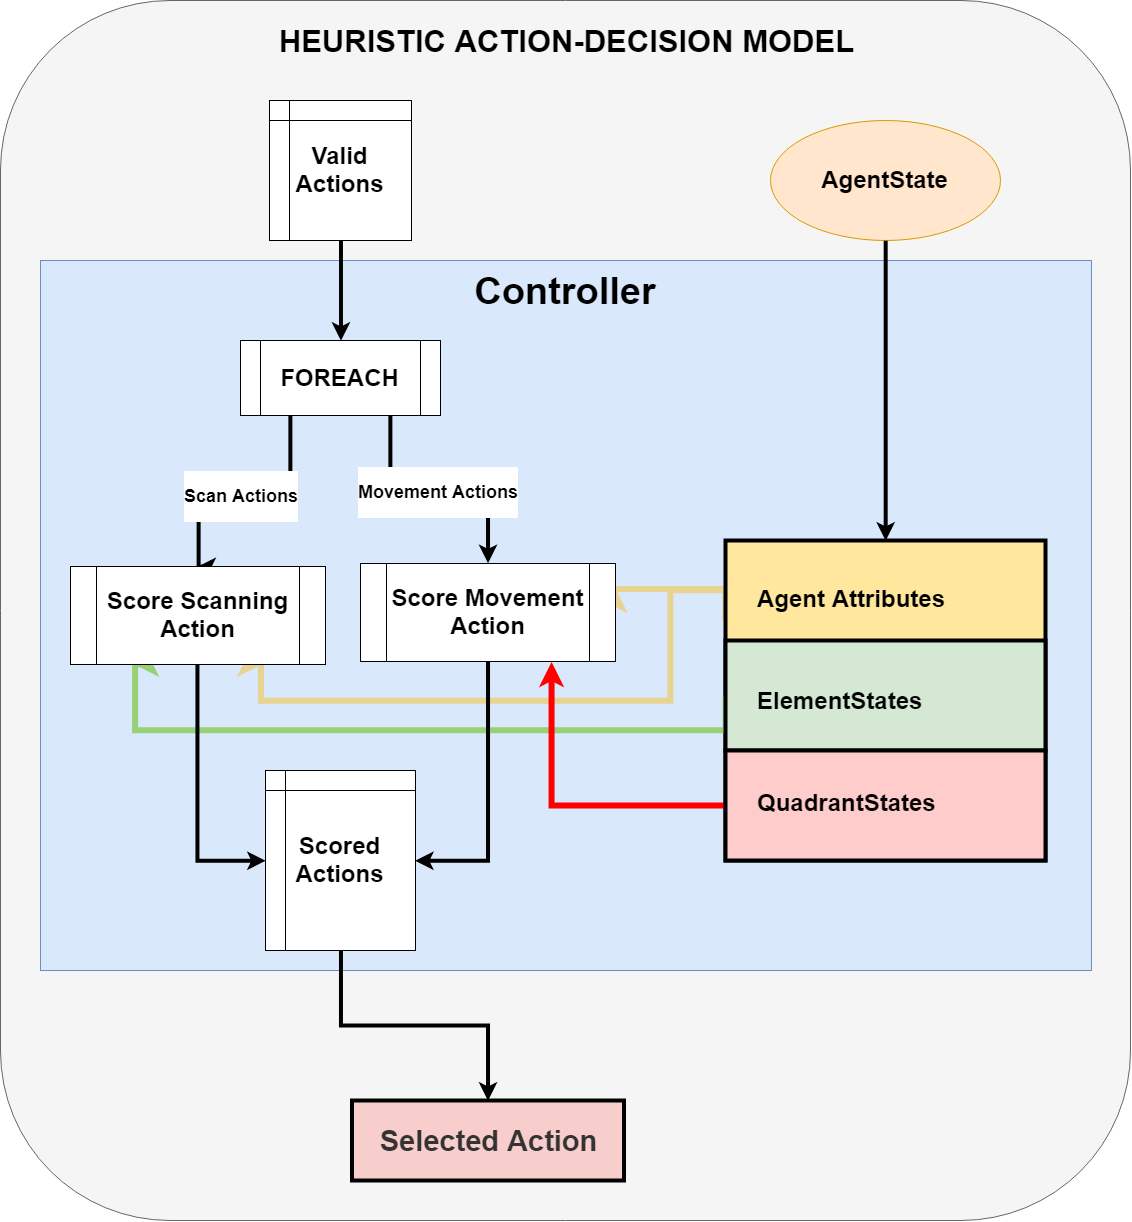
\includegraphics[width=1.0\columnwidth]{Figures/heuristic_decision_model.png}
  \caption{The general decision model that our heuristic controllers follow. An \texttt{AgentState} and a list of valid actions are passed to the controller. The controller then assigns a score to each action by analyzing related attributes within the \texttt{AgentState}. The highest scoring action is then returned.}
  \label{fig:heuristic_decision_model}
\end{figure}

Valid scanning actions are all scored using function~\ref{algorithmic:score_scan_action}.
Higher scores will be given to scanning actions for an element type that is considered more important and has fewer known values within the corresponding sensor's range.
Importance of an element type is determined by whether it is flagged as hazardous and/or as an indicator.
The amount of known values in the corresponding sensor's range is calculated by referencing the agent's \texttt{internalMap}.
The resulting score should influence the controller to use sensors efficiently, assist with hazard avoidance, and emphasize goal completion.

\begin{algorithm}[H]
  \setstretch{1.35}
  \caption{Calculate a score for a considered scanning action for a specific element type based on an \texttt{ElementState}. The returned result will be used to rank the action in the decision-making process. $W_{item}$ denotes the attributed weight for $itemReward$.}
  \begin{algorithmic} \label{algorithmic:score_scan_action}
    \REQUIRE $W_{indicator} \in \left[0, \infty \right)$
    \REQUIRE $W_{hazard} \in \left[0, \infty \right)$
    \REQUIRE $W_{pkir} \in \left[0, \infty \right)$
    \REQUIRE $W_{immediates} \in \left[0, \infty \right)$
    \REQUIRE $indicator \in \{true, false\}$
    \REQUIRE $hazard \in \{true, false\}$
    \REQUIRE $percentKnownInRange \in \left[0, 1 \right]$
    \REQUIRE $immediatesKnown \in \left[0, 4 \right]$
    \ENSURE $scanActionScore \in \left[0, 1 \right]$
    \IF {indicator = true}
      \STATE $iScore \leftarrow W_{indicator}$
    \ELSE
      \STATE $iScore \leftarrow 0$
    \ENDIF
    \IF {hazard = true}
      \STATE $hScore \leftarrow W_{hazard}$
    \ELSE
      \STATE $hScore \leftarrow 0$
    \ENDIF
    \STATE $pkirScore \leftarrow (1 - percentKnownInRange) \times W_{pkir}$
    \STATE $imdsScore \leftarrow ((4 - immediatesKnown) / 4) * W_{immediates}$
    \STATE $scoresTotal \leftarrow iScore + hScore + pkirScore + imdsScore$
    \STATE $W_{total} \leftarrow W_{indicator} + W_{hazard} + W_{pkir} + W_{immediates}$
    \RETURN $scanActionScore \leftarrow scoresTotal / W_{total}$
  \end{algorithmic}
\end{algorithm}


Scoring each valid movement actions is based on the controller's specific implementation of the \texttt{scoreMovmentAction} function.
These functions involve a series of sub-functions tied to each available sensor's element type.
Each of the sub-functions calculate a sub-score for their element type.
These sub-functions use threshold analyses on the \texttt{QuadrantState}s corresponding to the direction of movement being considered.
Once each element type's sub-score has been returned to the \texttt{scoreMovmentAction} function, an overall score is determined by a weighted average.
The overall scoring functions used for $Heuristic_{FH}$ (algorithm~\ref{algorithmic:findHuman_scoreMovmentAction}) and $Heuristic_{MW}$ (algorithm~\ref{algorithmic:mapWater_scoreMovementAction}) follow the same logic, but contain different sub-functions and related weights.
For an example of how threshold analyses are conducted within a sub-function, see $Heuristic_{FH}$'s \texttt{scoreElevation} algorithm (algorithm~\ref{algorithmic:findHuman_scoreElevation}).


\begin{algorithm}[H]
  \setstretch{1.35}
  \caption{Calculate a score for a considered movement action in a specific direction based on a set of corresponding \texttt{QuadrantState}s ($QS$). The returned results will be used to rank the action in the decision-making process. $W_{item}$ denotes the attributed weight for $itemReward$. This function also uses a $score<Element-Type>$ function. Example for one such equation is algorithm~\ref{algorithmic:findHuman_scoreElevation}. This equation is used specifically for the $Heuristic_{FH}$ controller's decision model.}
  \begin{algorithmic} \label{algorithmic:findHuman_scoreMovmentAction}
    \REQUIRE $W_{elevation} \in \left[0, \infty \right)$
    \REQUIRE $W_{decibel} \in \left[0, \infty \right)$
    \REQUIRE $W_{temperature} \in \left[0, \infty \right)$
    \REQUIRE $W_{water} \in \left[0, \infty \right)$
    \ENSURE $scoreElevation \rightarrow \left[0, 1 \right]$
    \ENSURE $scoreDecibel \rightarrow \left[0, 1 \right]$
    \ENSURE $scoreTemperature \rightarrow \left[0, 1 \right]$
    \ENSURE $scoreWater \rightarrow \left[0, 1 \right]$
    \ENSURE $movementActionScore \in \left[0, 1 \right]$
    \STATE $eScore \leftarrow scoreElevation(QS) * W_{elevation}$
    \STATE $dScore \leftarrow scoreDecibel(QS) * W_{decibel}$
    \STATE $tScore \leftarrow scoreTemperature(QS) * W_{temperature}$
    \STATE $wScore \leftarrow scoreWater(QS) * W_{water}$
    \STATE $scoresTotal \leftarrow eScore + dScore + tScore + wScore$
    \STATE $W_{total} \leftarrow W_{elevation} + W_{decibel} + W_{temperature} + W_{water}$
    \RETURN $movementActionScore \leftarrow scoresTotal / W_{total}$
  \end{algorithmic}
\end{algorithm}


\begin{algorithm}[H]
  \setstretch{1.35}
  \caption{Calculate a score for a considered movement action in a specific direction based on a set of corresponding \texttt{QuadrantState}s ($QS$). The returned results will be used to rank the action in the decision-making process. $W_{item}$ denotes the attributed weight for $itemReward$. This function also uses a $score<Element-Type>$ function. Example for one such equation is algorithm~\ref{algorithmic:findHuman_scoreElevation}. This equation is used specifically for the $Heuristic_{MW}$ controller's decision model.}
  \begin{algorithmic} \label{algorithmic:mapWater_scoreMovementAction}
    \REQUIRE $W_{elevation} \in \left[0, \infty \right)$
    \REQUIRE $W_{water} \in \left[0, \infty \right)$
    \ENSURE $scoreElevation \rightarrow \left[0, 1 \right]$
    \ENSURE $scoreWater \rightarrow \left[0, 1 \right]$
    \ENSURE $movementActionScore \in \left[0, 1 \right]$
    \STATE $eScore \leftarrow scoreElevation(QS) * W_{elevation}$
    \STATE $wScore \leftarrow scoreWater(QS) * W_{water}$
    \STATE $scoresTotal \leftarrow eScore + wScore$
    \STATE $W_{total} \leftarrow W_{elevation} + W_{water}$
    \RETURN $movementActionScore \leftarrow scoresTotal / W_{total}$
  \end{algorithmic}
\end{algorithm}


\begin{algorithm}[H]
  \setstretch{1.35}
  \caption{Calculate a score for a \texttt{QuadrantState} ($Q$) of element type ``elevation.'' The returned results will be used to rank the action in the decision-making process. $W_{item}$ denotes the attributed weight for $itemReward$. This equation is used in both the $Heuristic_{FH}$ and $Heuristic_{FH}$ controllers' decision models.}
  \begin{algorithmic} \label{algorithmic:findHuman_scoreElevation}
    \REQUIRE $W_{percentKnown} \in \left[0, \infty \right)$
    \REQUIRE $W_{immediateValue} \in \left[0, \infty \right)$
    \ENSURE $percentKnown \rightarrow \left[0, 1 \right]$
    \ENSURE $scanMovementScore \in \left[0, 1 \right]$
    \STATE $pkScore \leftarrow scoreElevation(QS) * W_{elevation}$
    \IF {$\exists immediateValue$}
      \IF {$|immediateValue| > 12$}
        \STATE $imScore \leftarrow 1$
      \ELSE
        \STATE $imScore \leftarrow 0$
      \ENDIF
    \ELSE
      \STATE $imScore \leftarrow 0$
    \ENDIF
    \STATE $scoresTotal \leftarrow pkScore + imScore$
    \STATE $W_{total} \leftarrow W_{elevation} + W_{decibel} + W_{temperature} + W_{water}$
    \RETURN $scanActionScore \leftarrow scoresTotal / W_{total}$
  \end{algorithmic}
\end{algorithm}


\section{SCOUt Controller} \label{sec:scout_controller}
The SCOUt controller uses reinforcement learning to build a memory of past actions and rewards for planning future actions.
After each operation, the SCOUt controller will store state-action rewards in memory.
A state-action reward (SAR) contains the action that the agent took, the state that the agent was in when it chose this action, and the short-term and long-term rewards that the agent received.
In future operations, the SCOUt controller (figure~\ref{fig:scout_decision_model}) will search in memory to find SARs with states that are similar to the agent's current state.
Utilizing data from the agent's current state and the controller's collection of past action-state pairs, SCOUt will predict rewards for each possible action and select one based on these predictions.

\begin{figure}[H]
  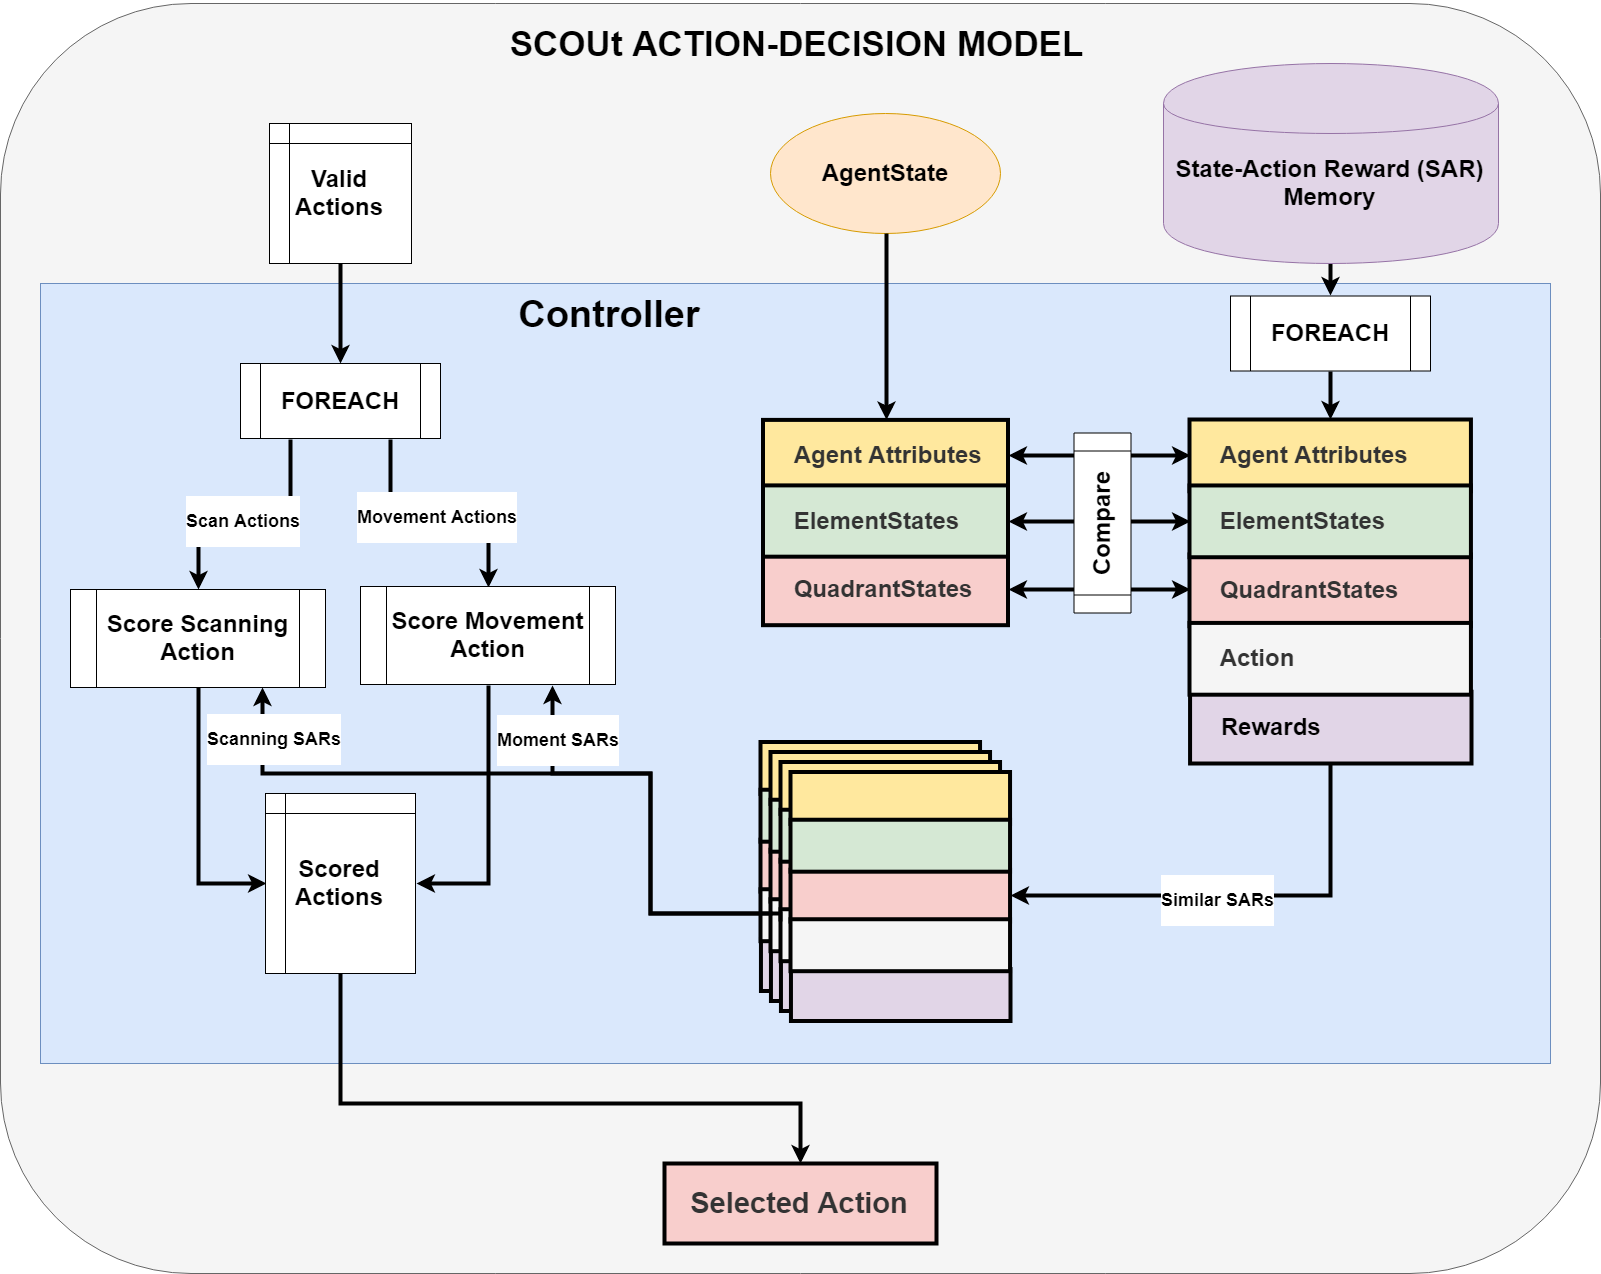
\includegraphics[width=1.0\columnwidth]{Figures/scout_decision_model.png}
  \caption{Action decision model for the SCOUt controller. The controller searches for memory state-action rewards (SAR) that have a similar state to the current state. The chosen actions and rewards for each similar SAR is used to create a score for each valid action that the can be taken in the current state.}
  \label{fig:scout_decision_model}
\end{figure}

Calculations used for action decision rely on several weights and variables to assist in state comparisons and future reward prediction.
Because of the large number of weights required for these calculations, a basic genetic algorithm (GA) was used to optimize these weights.
The GA initialized a population of 10 weight sets and evolved them for 50 generations.
Each generation creates five mutated copies and five crossover copies of individuals in the current population.
The individuals that are copied for mutation or crossover are chosen using roulette selection.
% \todo{ref roulette selection algo}
% \todo{ref GA algo}
Fitness scores are calculated for each of the resulting 20 individuals based on their performance within a series of 50 operations.
Ten survivors are then selected for the next generation.
Survivor selection keeps the two individuals with the highest fitness scores and uses roulette selection for choosing the remaining seven.
The weight set with the highest fitness in the final generation was selected for use in experimentation, and its values listed in table ~\ref{table:evolved_weight_set}.

% \todo{sizing}
\begin{table}
  \centering
  % \small
  \def\arraystretch{1.25}
  \caption{Set of variables and weights used by the SCOUt controller for action decision. These variables/weights were produced using a basic genetic algorithm.}
  \resizebox{\textwidth}{!}{%
  \begin{tabular}{ l l c }
    \textbf{Attribute}                & \textbf{Description}            & \textbf{Variable/Weight} \\
    \hline
                                      & \textbf{State Comparison Weights}& \\
    health                            & remaining health               & 0.41  \\
    energy                            & energy level                & 0.78  \\
    elementStates                     & overall element states                & 0.61  \\
    quadrantStates                    & overall quadrant states                & 0.16  \\
    \hline
                                      & \textbf{Element State Comparison Weights}& \\
    indicator                         & element type is indicator                & 0.31  \\
    hazard                            & element type is hazardous                & 0.07  \\
    percentKnownInRange               & known element type values in range of sensor                & 1.0   \\
    immediateKnown                    & number of immediate cell values known                & 0.41  \\
    \hline
                                      & \textbf{Quadrant State Comparison Weights}& \\
    indicator                         & element type is indicator                & 0.38  \\
    hazard                            & element type is hazardous                & 0.23  \\
    percentKnown                      & known element type values in quadrant                & 0.2   \\
    averageValue                      & average element value in quadrant cells                & 0.19  \\
    immediateValue                    & immediate quadrant cell value                & 0.29  \\
    \hline
                                      & \textbf{Action Selection}& \\
    similarityThreshold               & SAR comparison qualification  & 0.26  \\
    minimumSimilarStates              & used to calculate prediction ``confidence''    & 10    \\
    repetitionPenalty                 & penalty for action that would be repetitive                & 0.1   \\
    \hline
                                      & \textbf{Movement Action Score Weights}& \\
    predictedShortTermReward          & action's predicted short-term reward       & 0.87  \\
    predictedLongTermReward           & action's predicted long-term reward      & 0.45  \\
    confidence                        & confidence in predicted rewards       & 0.25  \\
    \hline
                                      & \textbf{Scanning Action Score Weights}& \\
    predictedShortTermReward          & action's predicted short-term reward       & 0.61  \\
    predictedLongTermReward           & action's predicted long-term reward      & 0.34  \\
    confidence                        & confidence in predicted rewards       & 1.0   \\
    \hline
  \end{tabular}}
  % \caption{Table ~\ref{table:evolved_weight_set}: Evolved Weight Set}
  \label{table:evolved_weight_set}
\end{table}


\subsection{Memory}
The SCOUt controller can gather memory from every operation.
When an operation has finished, and long-term rewards have been assigned to each action, the controller creates new SARs, and selects a sub-set of them to be stored in memory.
The rest are discarded.
Saving only a sub-set cuts back on the size of the memory file as well as the computational time that will be required to search for similar states.
The current memory selection method in this project's implementation saves the last 20 SARs, and a uniformly sampled sub-set of the remaining SARs from the operation.
The last 20 are always saved because they typically hold the most important events leading up to the success or failure of the operation.
To also capture events that occur during the agent's initial and intermediate search process, the controller retains 5 percent of the remaining SARs generated.
These SARs are uniformly sampled beginning at index 0.
So, if there were 100 SARs in the remaining set, SARs indexed 0, 20, 40, 60, and 80 would be stored in memory.
Each SAR is added to the controller's memory file as a JSON object.
The next time that the controller is used in operation, the collection of SARs can then be decoded from the file back into \texttt{StateActionReward} class instances.


\subsection{State Normalization}
The data within each SAR's state is relative to the operation in which they were recorded.
To handle variances found between all of the states stored in memory, SCOUt normalizes them using a Gaussian approach as suggested by McCaffrey~\cite{mccaffrey_how_nodate}.
Normalization helps make data values more meaningful when studied by the controller.
For example, if the controller was seeking out a human, it may look for increases in decibel values.
In order for the controller to determine how much of an increase is significant enough to investigate, it needs to first understand what variations are considered normal.
Gaussian distribution provides this functionality through the calculation of mean and standard deviation ($sd$) values in a data set.
If the agent has gathered decibel readings in its north quadrant that are well outside the $sd$ found in the controller's memory, it should be encouraged to investigate.
All numerical attributes within an \texttt{AgentState} are normalized using this Gaussian method.
This applies to health and \texttt{energyLevel} within \texttt{AgentState}s, \texttt{percentKnownInSensorRange} within \texttt{ElementState}s, and \texttt{percentKnown}, \texttt{averageValueDifferential}, and

\noindent
\texttt{immediateValueDifferential} within \texttt{QuadrantState}s.

The normalization process begins by extracting each of these attributes from all SAR states within the loaded memory.
Next the mean and standard deviation values are calculated and stored in an instance of a \texttt{GuassianData} class (Appendix~\ref{appendix:gaussian_data}).
Once mean and standard deviation values are known, the controller will go back through every SAR's state and normalize their attributes using each corresponding \texttt{GaussianData} class instance.
The normalization function (equation~\ref{eq:gaussian_normalize}) will produce a ``normal'' value that reflects how many standard deviations the attribute falls above or below the mean.
A value of 0 represents no difference between the attribute's value and the mean, values of 1 and -1 represent a difference of one standard deviation from the mean, and so on.
When SCOUt searches for similar states, it will also normalize the current state using the existing \texttt{GuassianData} instances.
By normalizing the current state against the states in memory, the numerical attributes compared will all be relative to the mean of the values held in memory.

\begin{capeq}
  \begin{equation} \label{eq:gaussian_normalize}
    x_{normal} = \frac{(x - m)}{sd}
  \end{equation}
  \caption{Normalization of an attribute value, $x$, based on the gaussian mean, $m$, and gaussian standard deviation, $sd$, for the given attribute.}
\end{capeq}


% \todo{major revisions to this section}
% Replace as much as possible with graphics
% \todo{eliminate weighted average refs?}

\subsection{State Comparisons} \label{subsec:state_comparisons}
Now that all state attributes are normalized, the controller can use a more intuitive approach for calculating the differences between two states.
State comparisons are used to build a set of SARs from memory that contain states similar to an agent's current state.
These SARs will later be used to assist in reward prediction.
For an SAR to qualify for addition into this set, its state must have an overall difference below the \textit{similarityThreshold} specified in table ~\ref{table:evolved_weight_set}.
Overall state difference is calculated using a series of difference calculations between related attributes in the two compared \texttt{AgentState}s.
Results from the series of difference calculations will all be collapsed into a single \textit{overallStateDifference} using a weighted average function (equation ~\ref{eq:weighted_average}).
By comparing each attribute separately and applying a weighted average to the resulting difference calculations, this allows the controller to assign a level of importance to each individual attribute.
Importance is assigned via weight values that are between 0 and 1 (see ``state comparison'' weights in table~\ref{table:evolved_weight_set}).
The higher the attribute's weight it, the more influence it will have in the overall state difference.
An attribute with a weight of 0 will be completely ignored in a weighted average equation.
Different weighted average equations are used for \textit{overallStateDifference} calculation depending on whether the considered SAR's action is a movement or scanning action.
This allows the controller to compare only the attributes that are relevant to the type of action that was selected.

\begin{capeq}
  \begin{equation} \label{eq:weighted_average}
    WeightedAverage = \frac{\sum_{i=0}^{n} A_{i} * W_{i}}{\sum_{i=0}^{n} W_{i}}
  \end{equation}
  \caption{A general equation that takes a list of $n$ attribute values ($V$) and a list of $n$ corresponding weights ($W$) and calculates a weighted average of all attribute values.}
\end{capeq}

Difference comparisons for each attribute in an \texttt{AgentState} are calculated based on their data type (boolean, normalized numerical value, optional normalized numerical value, or sub-class).
Sub-class comparisons, such as comparing two \texttt{ElementState}s, follow the same procedure as \texttt{AgentState} does for calculating an overall difference.
Difference comparisons will be made for each of the attributes within the sub-class, and a weighted average function is applied to the results.
Boolean differences will return 0 when the compared attributes are both true or both false and return 1 otherwise (equation ~\ref{eq:boolean_difference}).
For example, \textit{BooleanDifference} is used to calculate whether an element type in two \texttt{ElementState}s were both flagged as an indicator or not.
Normalized numerical attributes follow the \textit{GaussianDifference} equation (equation ~\ref{eq:gaussian_difference}).
This equation will produce values that hold the same principle as the normalization process, where the closer the difference is to 0, the more similar they are.
If two values are identical, their \textit{GaussianDifference} will be 0.
Otherwise, the \textit{GaussianDifference} will be relative to how many standard deviations away from each other the two values are.
% Proofs for these behaviors are found in appendix item~\ref{appendix:gaussian_difference_identical} and appendix item~\ref{appendix:gaussian_difference_different} respectively.
Optional values follow a unique case-based equation (equation~\ref{eq:option_difference}) to calculate the \textit{GuassianDifference} only when both are known.
If one value is known and the other is not, a difference of 1 is returned.
If both values are unknown a difference of 0 is returned.

\begin{capeq}
\begin{equation} \label{eq:boolean_difference}
  BooleanDifference = \begin{cases}
    x = y & 0 \\
    x \neq y & 1
  \end{cases}
\end{equation}
\caption{Difference calculation for two boolean values, $x$ and $y$.}
\end{capeq}

\begin{capeq}
\begin{equation} \label{eq:gaussian_difference}
  GaussianDifference = |x_{normal} - y_{normal}|
\end{equation}
\caption{Difference calculation for two normalized vales, $x$ and $y$.}
\end{capeq}

\begin{capeq}
\begin{equation} \label{eq:option_difference}
  optionDifference =
  \begin{cases}
    x \quad \text{known} \cap y \quad \text{known} & GaussianDifference(x,y) \\
    x \quad \text{known} \oplus y \quad \text{known} & 1 \\
    x \quad \neg \text{known} \cap y \quad \neg \text{known} & 0
  \end{cases}
\end{equation}
\caption{A difference calculation used for two values ($x$ and $y$), when their values are not always known.}
\end{capeq}

Comparisons with SAR's whose chosen action was a scanning action will apply a weighted average to the health, energy, and element states of the two \texttt{AgentState}s.
Each \texttt{ElementState} within the current \texttt{AgentState} will calculate their own weighted average based on the number of the immediately adjacent cells that are known, the percent of known element values in range of the sensor, the hazard and indicator flags.
All of these \textit{elementStateDifference}s will be averaged (non-weighted) into a single difference value, \textit{averageElementStateDifference}.
This compares the usage of the element type (hazard and/or indicator detection), and knowledge of the element type (percent known within the environment).
The \textit{hazard} and \textit{indicator} differences can help the controller determine the usage of the element type's data being collected.
The \textit{percentKnown} and \textit{immediateValuesKnown} differences help the controller decide whether use of an element type's sensor is efficient or necessary.
For example, if an agent does not have knowledge of the elevation in adjacent cells, it couldn't confidently determine whether it is safe or possible to move into one of those cells without first scanning to find out.

% \begin{capeq}
%   \begin{align*}
%   \begin{equation} \label{eq:scanning_overall_difference}
%     &V = \{health_{diff},\quad energy_{diff},\quad elementStates_{diff}\} \\
%     &W = \{health_{wight},\quad energy_{wight},\quad elementStates_{wight}\} \\
%     &\\
%     &OverallDifference_{s} = WeightedAverage(V,W)
%   \end{equation}
% \end{align*}
% \caption{Calculation for the overall state difference when the compared state-action reward had chosen a scanning action, where $V$ is a list of attributes values and $W$ is the list of weights for the attributes.}
% \end{capeq}

% \begin{capeq}
% \begin{equation} \label{eq:element_state_difference}
% % \begin{align*}
%   &V = \{indicator_{diff},\quad hazard_{diff},\quad percentKnownInRange_{diff},\quad immediateKnown_{diff}\} \\
%   &W = \{indicator_{wight},\quad hazard_{wight},\quad percentKnownInRange_{wight},\quad immediateKnown_{weight}\} \\
%   &\\
%   &elementStateDifference = WeightedAverage(V,W)
% % \end{align*}
% \end{equation}
% \caption{Calculation for the overall difference of two \texttt{ElementState}s, where $V$ is a list of attributes values within the \texttt{ElementState}s and $W$ is the list of corresponding weights.}
% \end{capeq}

If the SAR's action type is movement, overall state difference is calculated using differences in each \texttt{AgentState}s' health, energy, element states, and quadrant states.
In addition to calculating \textit{elementStateDifference}s, \textit{quadrantToQuadrantDifferences} are calculated between every quadrant in the current state and every quadrant in the SAR state.
Only one ``orientation'' of quadrant-to-quadrant comparisons will be used in the overall difference calculation.
Four orientations are considered by rotating the SAR's quadrants in 90 degree intervals (see figure ~\ref{fig:quadrant_orientations}).
The resulting orientation comparisons are denoted as North-to-North, North-to-West, North-to-South and North-to-East (based on the SAR's quadrant that is matched to the current state's North quadrant).
The orientation that yields the lowest \textit{quadrantToQuadrantDifferences} (\textit{lowestQuadrantOrientationDifference}) is used in calculating $OverallDifference_{m}$.

% \begin{capeq}
% \begin{equation} \label{eq:movement_overall_difference}
% \begin{align*}
%   &V = \{health_{diff},\quad energy_{diff},\quad elementStates_{diff},\quad quadrantStates_{diff}\} \\
%   &W = \{health_{wight},\quad energy_{wight},\quad elementStates_{wight},\quad quadrantStates_{weight}\} \\
%   &\\
%   &OverallDifference_{m} = WeightedAverage(V,W)
% \end{align*}
% \end{equation}
% \caption{Calculation for the overall state difference when the compared state-action reward had chosen a movement action, where $V$ is a list of attributes values and $W$ is the list of weights for the attributes.}
% \end{capeq}

\begin{figure}[H]
  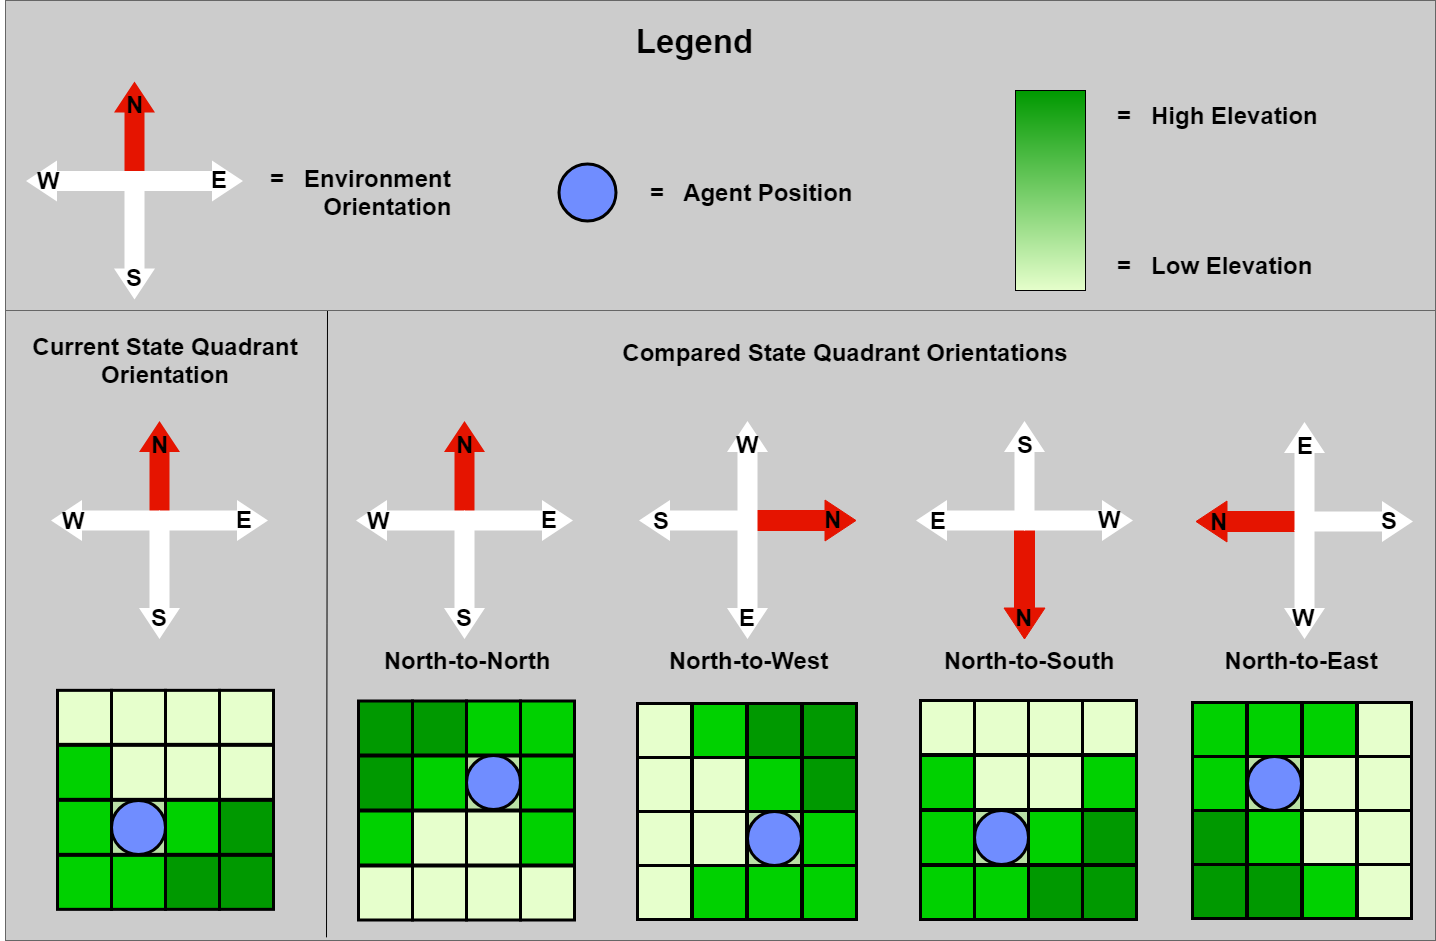
\includegraphics[width=1.0\columnwidth]{Figures/quadrant_orientations.png}
  \caption{Orientation considerations between two compared states. This displays how rotating the compared environment's quadrant orientation can reveal states of higher similarity. We see that the elevation heatmaps of the two are highly similar when compared at North-to-South orientation, where as an un-altered quadrant comparison (North-to-North) would yield a very negative comparison.}
  \label{fig:quadrant_orientations}
\end{figure}

Each orientation is important to consider because the controller is only concerned with moving towards interesting features in an environment, regardless of the direction.
Considering the orientation with the lowest difference makes the comparison relative to the two environments instead of the cardinal direction.
Consider if a highly similar SAR held information that its agent received good rewards for a particular movement action.
The current agent should be encouraged to move towards the quadrant in its own environment that holds similar features (not necessarily in the same direction).
Now, if the SAR's \textit{lowestQuadrantOrientationDifference} is found when rotating its quadrants 180 degrees (North-to-South orientation) and it had chosen to move East, the current agent should choose to move West since the two states are oriented at a 180 degree difference between each other (see figure ~\ref{fig:oriented_movement_example}).

\begin{figure}[H]
  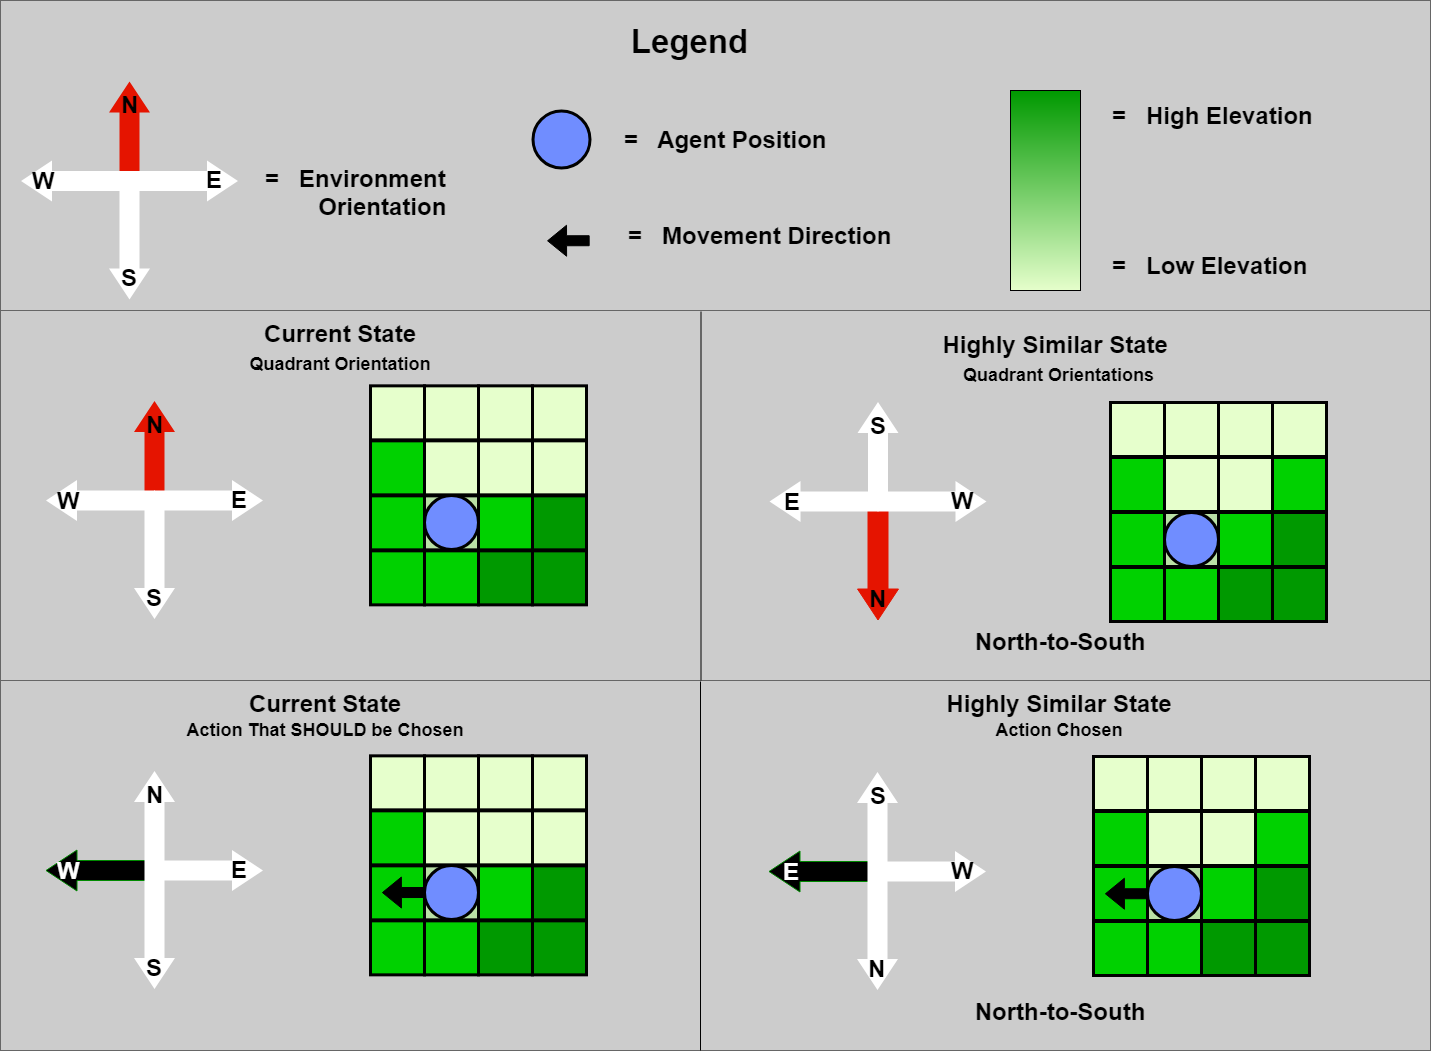
\includegraphics[width=1.0\columnwidth]{Figures/oriented_movement_example.png}
  \caption{Example of two states that have a \textit{lowestQuadrantOrientationDifference} at North-to-South orientation. The display exemplifies how after finding the most similar orientation, the action taken by the compared state must also be re-oriented to match the \textit{lowestQuadrantOrientationDifference}. In doing so the agent will be considering movement relative to the matching features in the environment.}
  \label{fig:oriented_movement_example}
\end{figure}

Quadrant-to-quadrant comparisons produce a non-weighted average of \textit{quadrantElementStateDifference}s.
A \textit{quadrantElementStateDifference} is calculated between every \texttt{ElementState} in the current state's considered quadrant and the matching \texttt{ElementState} in the SAR state's considered quadrant (if it exists).
The \textit{quadrantElementStateDifference} uses a weighted average to compare attributes within the two \texttt{ElementState}s' considered quadrants.
For example, making a North-to-South quadrant comparison would consider element types in the current state's North quadrant against element types in the SAR's South quadrant.
When making these comparisons, it is not guaranteed that the current state and SAR state will share all the same element types.
For example, if the current state contains decibel data and the SAR state does not, no comparison can be made, and it will receive a \textit{quadrantElementStateDifference} of 1.
Because we are only comparing against element types in the current \texttt{AgentState}, if the SAR contains any element types not present in the current state, they are simply ignored.
These comparisons examine how much information about the element type is known, and the actual values in the quadrants (if they are known).
Because \texttt{averageValueDifferential} and \texttt{immediateValueDifferential} are not guaranteed to be known values for every quadrant, they use the unique option difference equation (equation ~\ref{eq:option_difference}).

% \begin{capeq}
% \begin{equation} \label{eq:quadrant_element_state_difference}
% \begin{align*}
%   &V = \{percentKnown_{diff},\quad averageValueDifferential_{diff},\quad immediateValueDifferential_{diff}\} \\
%   &W = \{percentKnown_{wight},\quad averageValueDifferential_{wight},\quad immediateValueDifferential_{wight}\} \\
%   &\\
%   &quadrantElementStateDifference = WeightedAverage(V,W)
% \end{align*}
% \end{equation}
% \caption{Calculation for comparing the difference between two \texttt{ElementState}s in given quadrants, where $V$ is a list of attributes values and $W$ is the list of weights for the attributes.}
% \end{capeq}

Once all sub-differences have been calculated and either $OverallDifference_{s}$ or $OverallDifference_{m}$ is known, the controller can decide whether the SAR qualifies to be used in future reward prediction for the current agent.
If the calculated overall difference is below the \textit{similarityThreshold}, the SAR will qualify and an instance of the \texttt{StateActionDifference} class (Appendix~\ref{appendix:state_action_difference}) is created.
Each instance stores the overall difference value, the SAR's action taken, and the short-term and long-term rewards.
State comparison will be repeated for every SAR in the memory pool, and the resulting collection of \texttt{StateActionDifference} instances is passed to the action reward prediction algorithm.



\subsection{Action Reward Prediction}
Once the controller has generated a set of \texttt{StateActionDifference}s (SAD), it will predict a short-term and long-term reward value that each possible action might receive, along with a confidence score for the predictions.
For each valid action considered, the algorithm will select a sub-set of SAD where the \texttt{StateActionDifference}'s \texttt{action} is the same as the one being considered.
Predicted short-term and long-term rewards are calculated as an average of all the \texttt{shortTermScore}s and \texttt{longTermScore}s in the sub-set.
Confidence is evaluated using the average of the \texttt{overallStateDifference}s in the sub-set, weighted by the number of \texttt{StateActionDifference}s in the sub-set (equation~\ref{eq:confidence}).
The equation will invert \textit{overallStateDifference}s when averaging them by subtracting their value from 1 (equation~\ref{eq:diff_to_similarity}).
This allows the prediction algorithm to look at them as ``similarity'' scores instead of ``difference'' scores.
If the overall difference had been 0 (the states compared were identical), their similarity score will be 1.
Because \textit{similarityThreshold} was used to filter out SARs with high overall difference values, it can be asserted that the average of all \textit{overallStateDifference}s will not fall below: $1 - similarityThreshold$.
The prediction algorithm then computes an overall \textit{actionScore} for each action using a weighted average of the predicted short-term reward, predicted long-term reward, and the confidence score.

\begin{capeq}
\begin{equation} \label{eq:diff_to_similarity}
  similarity = 1 - difference
\end{equation}
\caption{Equation for inverting an \textit{overallStateDifference} value to create a similarity value. The minimum \textit{overallStateDifference} that can exist is 0. By this logic, the highest attainable similarity between two states is 1.}
\end{capeq}

\begin{capeq}
\begin{equation} \label{eq:confidence}
  confidence = \begin{cases}
    n = 0 & 0 \\
    n < minimumSimilarStates & \frac{\sum_{n}^{i=0} 1 - SAD_{i}.overallStateDifference}{minimumSimilarStates} \\
    n >= minimumSimilarStates & \frac{\sum_{n}^{i=0} 1 - SAD_{i}.overallStateDifference}{n} \\
\end{cases}
\end{equation}
\caption{Confidence value assigned to reward prediction values based on a set of $n$ \texttt{StateActionDifference}s ($SAD$), and the $minimumSimilarStates$ value from the evolved weight set (table ~\ref{table:evolved_weight_set}).}
\end{capeq}

% \begin{capeq}
% \begin{equation} \label{eq:action_score}
% \begin{align*}
%   &V = \{predictedShortTermReward,\quad predictedLongTermReward,\quad confidence\} \\
%   &W = \{predictedShortTermReward_{weight},\quad predictedLongTermReward_{weight},\quad confidence_{weight}\} \\
%   &\\
%   &actionScore = WeightedAverage(V,W)
% \end{align*}
% \end{equation}
% \caption{Action scoring function using the action's $predictedShortTermReward$, $predictedLongTermReward$, and $confidence$, in pairing with their corresponding weights found in table ~\ref{table:evolved_weight_set}}
% \end{capeq}


\subsection{Action Selection}
Once every valid action has received an \textit{actionScore}, there are two methods the controller may use for choosing which one the agent should perform.
If the controller is being trained, roulette selection is used.
Roulette selection is an integral part of training as it will give every action a chance to be selected.
This will fill the controller memory with a variety of events both good and bad, giving the reward prediction algorithm more concise data to work with.
When the controller is being used outside of training, the action with the highest score is always selected.
Once selected, the agent will then attempt to perform the action, and its interaction with the environment will be reflected in a new \texttt{AgentState}.
If the agent is still operational after the resulting event and the goal has not yet been completed, the action decision process (figure ~\ref{fig:scout_decision_model}) will begin again using the new \texttt{AgentState}.
Once the agent is no longer operational, or the goal has been completed, the operation process ends, and new SARs are added to the controller's memory file.







% \todx{style algo}
% \begin{lstlisting}
% 1. Normalize the current state (how many SDs it falls outside of the average)
% 2. Calculate the Gaussian difference for:
%   a. health
%   b. energyLevel
%   c. elementStateDifferences = for each element state:
%     i. hazardDifference = if (current == SAR) 1 else 0
%     ii. indicatorDifference = if (current == SAR) 1 else 0
%     iii. percentKnownInSensorRangeDifference = abs(SAR - current)
%     iv. immediateValuesKnownDifference = abs(SAR - current) / 4
%   d. quadrantToQuadrantStateDifferences = for each current quadrant:
%     i. quadrantStateDifferences = for each SAR quadrant:
%       a. quadrantElementStateDifferences = for each element type:
%         i. hazardDifference = if (current == SAR) 1 else 0
%         ii. indicatorDifference = if (current == SAR) 1 else 0
%         iii. percentKnownDifference = abs(SAR - current)
%         iv. averageValueDifferentialDifference = if (current known && SAR known) abs(SAR - current) else (if current known == if SAR knonw) 1 else 0)
%         v. immediateValueDifferentialDifference = if (current known && SAR known) abs(SAR - current) else (if current known == if SAR knonw) 1 else 0)
% 3. Sum all differences together using weighted values for each Gaussian difference.
%   a. Movement state difference
%   b. Scan state difference
% \end{lstlisting}



% \subsection{Action Reward Prediction}
% Action reward prediction first calculates three factors for each valid action being considered: predicted short term reward, predicted long term reward and confidence.
% These factors are determined by StateActionDifference that hold the same action as the current action whose reward is being predicted.
% Only a list of similar StateActionDifferences are considered in these calculations.
% This list is made up of StateActionDifferences with an overall difference below a the set minDifferenceThreshold.
% Predicted short and long term rewards are calculated by the average of short and long term scores within the list of similar StateActionDifferences.
%
% If there are no StateActionDifferences in the list, the action being considered will receive a predicted short term reward and long term reward of 0.5 and a confidence of 0.


% An action's short and long term rewards are predicted from the averages of SARs where: A) the considered action was selected, and B) the state difference from the current state is below a certain threshold.
% In addition to these predicted rewards, we also calculate a confidence value for the predictions.
% \tods{confidence EQ}
% The lower the difference is between the current and SAR states, the higher the confidence will be.
% Additionally, the more SARs that are considered in the prediction, the more confident the controller can be in the predicted reward.
